% !TEX TS-program = pdflatex
% !TEX encoding = UTF-8 Unicode

% This is a simple template for a LaTeX document using the "article" class.
% See "book", "report", "letter" for other types of document.

\documentclass[12pt]{article} % use larger type; default would be 10pt

\usepackage[utf8]{inputenc} % set input encoding (not needed with XeLaTeX)

%%% Examples of Article customizations
% These packages are optional, depending whether you want the features they provide.
% See the LaTeX Companion or other references for full information.

%%% PAGE DIMENSIONS
\usepackage{geometry} % to change the page dimensions
\usepackage{latexsym}
\usepackage{mathabx}
\usepackage{ltablex}
\geometry{a4paper} % or letterpaper (US) or a5paper or....
% \geometry{margin=2in} % for example, change the margins to 2 inches all round
% \geometry{landscape} % set up the page for landscape
%   read geometry.pdf for detailed page layout information

\usepackage{graphicx} % support the \includegraphics command and options
\usepackage{longtable}
\usepackage{mdwlist}
% \usepackage[parfill]{parskip} % Activate to begin paragraphs with an empty line rather than an indent

%%% PACKAGES
\usepackage{booktabs} % for much better looking tables
\usepackage{array} % for better arrays (eg matrices) in maths
\usepackage{paralist} % very flexible & customisable lists (eg. enumerate/itemize, etc.)
\usepackage{verbatim} % adds environment for commenting out blocks of text & for better verbatim
\usepackage{subfig} % make it possible to include more than one captioned figure/table in a single float
% These packages are all incorporated in the memoir class to one degree or another...

%%% HEADERS & FOOTERS
\usepackage{fancyhdr} % This should be set AFTER setting up the page geometry
\pagestyle{fancy} % options: empty , plain , fancy
\renewcommand{\headrulewidth}{0pt} % customise the layout...
\lhead{}\chead{}\rhead{}
\lfoot{}\cfoot{\thepage}\rfoot{}

%%% SECTION TITLE APPEARANCE
\usepackage{sectsty}
\allsectionsfont{\sffamily\mdseries\upshape} % (See the fntguide.pdf for font help)
% (This matches ConTeXt defaults)

%%% ToC (table of contents) APPEARANCE
\usepackage[nottoc,notlof,notlot]{tocbibind} % Put the bibliography in the ToC
\usepackage[titles,subfigure]{tocloft} % Alter the style of the Table of Contents
\usepackage{listings}
\usepackage{color}
\lstset{emph={%
    WhenEver, WhenFingerDownOn, WhenFingerUpOn, WhenFingerMovesOn,
    WhenIntegerChanges,
    WhenCollisionBetween, NoCollisionBetween, NoCollisionEffectBetween,
    class, extends, import, var%
    },
    emphstyle={\bfseries},%
    escapeinside={(*}{*)}, 
}%
% "define" Scala
\lstdefinelanguage{scala}{morekeywords={class,object,trait,extends,with,new,if,while,for,def,val,var,this},
otherkeywords={->,=>},
sensitive=true,
morecomment=[l]{//},
morecomment=[s]{/*}{*/},
morestring=[b]"}
\definecolor{dkgreen}{rgb}{0,0.6,0}
\definecolor{gray}{rgb}{0.5,0.5,0.5}
\definecolor{mauve}{rgb}{0.58,0,0.82}
 
% Default settings for code listings
\lstset{
  language=scala,
  aboveskip=3mm,
  belowskip=3mm,
  showstringspaces=false,
  columns=flexible,
  basicstyle={\small\ttfamily},
  numbers=none,
  numberstyle=\tiny\color{gray},
  keywordstyle=\color{blue},
  commentstyle=\color{dkgreen},
  stringstyle=\color{mauve},
  frame=single,
  breaklines=true,
  breakatwhitespace=true
  tabsize=3
}

\renewcommand{\cftsecfont}{\rmfamily\mdseries\upshape}
\renewcommand{\cftsecpagefont}{\rmfamily\mdseries\upshape} % No bold!

%%% END Article customizations

%%% The "real" document content comes below...

\title{King Pong Designer - Online Graphical Rule-Based Game Programming on
Tablets}
\author{Mikaël Mayer \\
   Supervisor: Viktor Kuncak \\
   Laboratory of Automated Reasoning and Analysis,\\
   EPFL, Lausanne, Switzerland \\
   \texttt{mikael.mayer@epfl.ch}}
%\date{} % Activate to display a given date or no date (if empty),
         % otherwise the current date is printed 
\bibliographystyle{alpha}
\begin{document}
\maketitle
\abstract{King Pong Designer is an innovative game engine which allows users to
graphically and completely interactively program multi-touch games on tablets
like multi-player Pong, Brick-breaker, Pacman and many others. It allows
programming mostly using only a finger by combining implicit and explicit
features.
We are looking forward to use this game engine for educational and entertaining purposes.}

\section{Introduction}

The way most people program is by writing explicit code,
which gets compiled to binary code. The use of libraries allows to reduce the
burden of specifying every single program behavior. Several programming
languages allow the user to have high-level structures, such as object-oriented
languages, partial functions or even constraint programming. But a lot of time
is still spent writing programs without seeing the result immediately. This is
why we tried a different approach to programming that makes it easier.

In this report, we present our game engine named King Pong Designer.
King Pong Designer is an innovative game engine which allows users to
graphically and completely interactively program multi-touch games like
multi-player Pong, brick-breaker, Pacman and many others. Its interaction is
finger-based and through backtracking mechanisms allows programming by finger
by combining implicit and explicit features.

\begin{figure}[h]
\centering
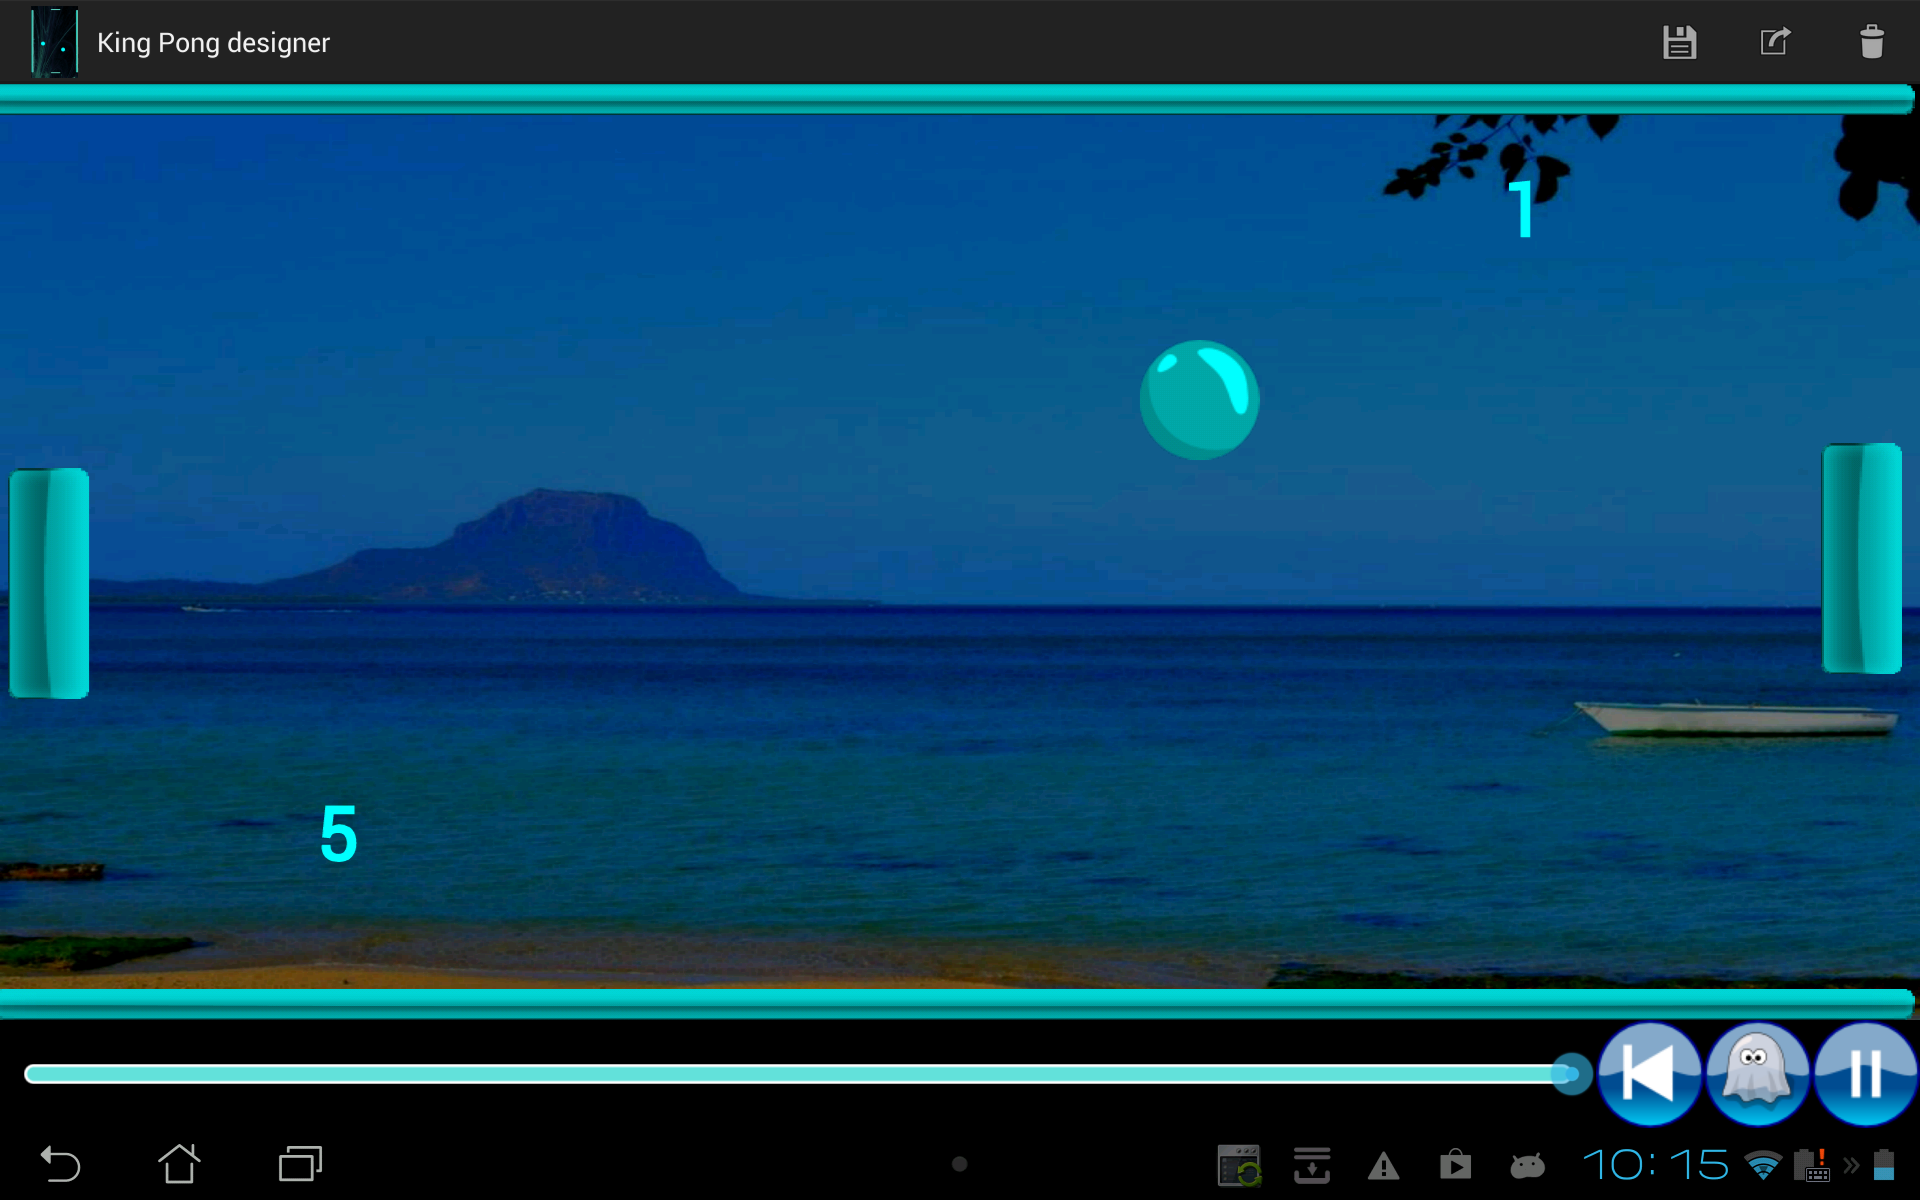
\includegraphics[width=5in]{captures/PongGame}
\caption{The two-player game of Pong in our game engine\label{ponggame}}
\end{figure}
\begin{figure}
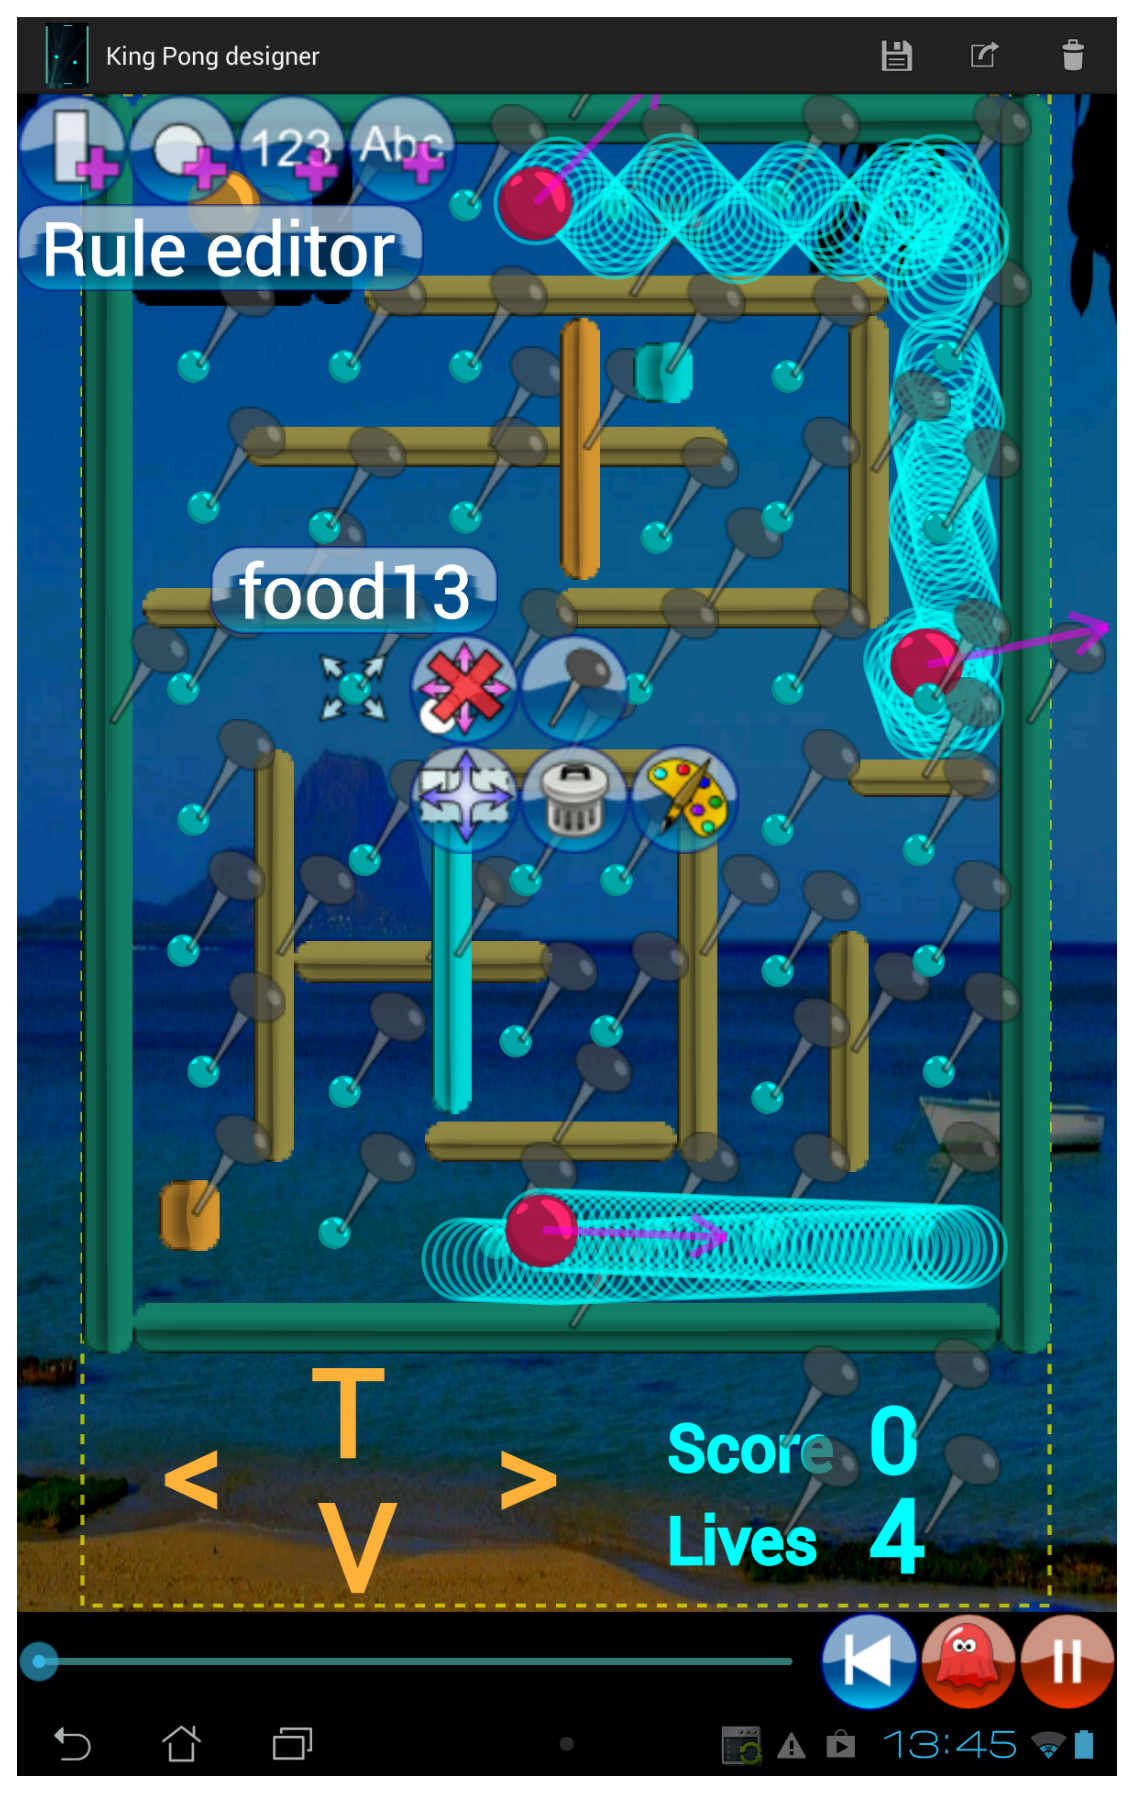
\includegraphics[width=5in]{captures/PacmanGhostMode}
\caption{Time History in the Pacman game\label{pacman}}
\end{figure}

\section{Related Work}

Modern programming languages, like Kaplan for Scala
\cite{koksal_constraints_2012} or Comfusy \cite{kuncak_comfusy:_2010}, start to
adopt the use of constraint programming structures. Such structures allow
programmers to work productively on explicit specifications rather than
explicit code. The automatically generated code is thus less error-prone.
Decreasing the number of potential errors is also the goal of Domain-specific
languages like those designed by Intentional Programming
\cite{simonyi_intentional_2006}, which allows the programmer to work on a
language that is closer to his needs.
Our game engine has also a domain-specific rule-based language that is
generated by the graphical selections made by the user.

The idea of programming graphically has already inspired some people to
design functional GUI programming \cite{elliott_genuinely_2001}. Our
graphical approach is comparatively more state/rule-based rather than
function-oriented.

Quickdraw \cite{cheema_quickdraw:_2012} is a graphical system whichs
rebuilds precise graphics based on vague input. It inspired us to
enforce the robustness of our system against minor graphics specification errors.

The way we handle objects and context menus is very similar to the educational
object-oriented framework Squeak \cite{sanchez-ruiz_funfonts:_2008}. Its
specificity is to make the interaction more user-friendly by being able to
modify the game state on-the-fly.

The way our game engine is designed is basically comparable to the one in
\cite{bishop_designing_1998} but less complex. For example, our
collision engine only detects static collisions, not dynamic ones.

Modern debuggers allow the possibility of going back in time to solve complex
problems
\cite{ko_debugging_2008}. Similarly, our system uses time-backtracking to be
able to design and modify rules precisely.

Our constraint system is mostly based on input-output examples provided by the
user and generalized by the system, an approach that has been
explored by Gulwani et al.
\cite{singh_synthesizing_2012,gulwani_synthesis_2012}

The way the rules are refined according to multiple input-output examples is
similar to the Version Space Algebra method which automatically learns 
programs from trace \cite{lau_learning_2003}. Is also related to that
process the Angelic nondeterminism \cite{bodik_programming_2010}, which also
provides a methodology to fill the missing parts of code based on trace
executions and specifications.

The problem of merging
multiple states during symbolic execution found in
\cite{kuznetsov_efficient_2012} is similar to the problem of merging game
changes to one single rule.

Assisting the programmer to choose the best code according to specifications
\cite{shacham_chameleon:_2009} inspired us to do our semi-automatic rule
generator where the user can choose the code that matches its specifications, if
multiple code possibilities were found. If specifications consist in the
code context and the type of the current expression, such
interactive code suggestions based on types has also been explored in
\cite{gvero_interactive_2011}.

Finally, the way to manage coexistence between the code and its execution
has been already source of many more or less fruitful experiments. The
Khan Academy
\cite{sal_khan_2012} focuses more on ``play with the code'' than on its graphical
output, which is vigorously criticized by \cite{bret_learnable_2012}. Our approach
incorporates many important points of the second reference to make graphical
programming enjoyable.



\section{Lessons learned in this project}
Our initial purpose was to create an interface that the user can program
both graphically and/or with a text editor, with a preference to the first.
During programming, we also learned a lot by recording bugs and interesting
mistakes in the code, that might be used for future research.

Many upcoming challenges were not obvious at the beginning. First, what did we
mean by graphical programming? How would we make it at least Turing-complete?
What could be the purpose of it?

We will first introduce the challenges we had when designing the interface, then
concerning the implicit and explicit user interaction, and then how to link the
graphical and application programming interfaces by bootstrapping.


\begin{figure}
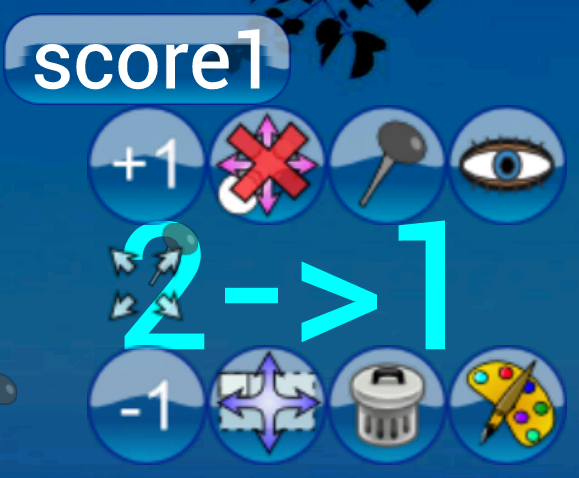
\includegraphics[height=2in]{captures/score2to1}
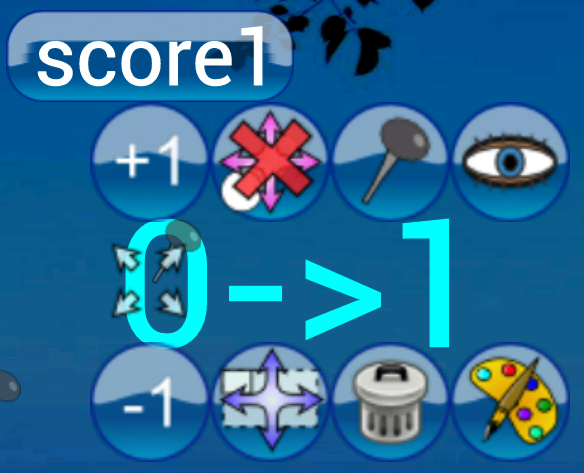
\includegraphics[height=2in]{captures/score0to1}

\begin{lstlisting}[language=scala]
WhenIntegerChanges(score) { (oldValue, newValue) =>
  if(newValue == 5) {
    score1.value += -1 || score1.value = 1
  }
}
WhenIntegerChanges(score) { (oldValue, newValue) =>
  if(newValue >= 0) {
    score1.value += 1 || score1.value = 1
  }
}
\end{lstlisting}

(a.) Incoherent way of merging rules :
\begin{lstlisting}[language=scala]
WhenIntegerChanges(score) { (oldValue, newValue) =>
  if(newValue == 5) {
    score1.value += -1 || score1.value = 1
  }
  if(newValue >= 0) {
    score1.value += 1 || score1.value = 1 //Double modification /!\
  }
}
\end{lstlisting}

(b.) Coherent way of merging rules :
\begin{lstlisting}[language=scala]
WhenIntegerChanges(score) { (oldValue, newValue) =>
  if(newValue <= -1) {
  } else if(newValue == 5) {
    score1.value = 1 // Merged code
  } else {
    score1.value += 1 || score1.value = 1
  }
}
\end{lstlisting}
\caption{Problem while merging two integer rules\label{differentrules}}
\end{figure}

\subsection{Designing the interface}



We first came up with the idea of programming a multi-player game of Pong (see
Figure \ref{ponggame}) in the following way. The user adds a moving ball, two
walls, two paddles and two scores. To add game logic, she would run the
simulation, add some input, pause the simulation, and specify rules modifying
the game according to events and inputs.



Another challenge was to choose the platform. Instead of making it web-based
or computer-based, we decided to implement our game engine on an Android
tablet with the Android SDK. That way, we could use a simple finger-based
interface, and our game could benefit from the multi-touch capabilities of the
device to make multi-player games.

Later, as we were designing the API and GPI (Graphical Programming Interface),
we faced the problem of storing the state of the game throughout the time, to be
able to come back. After testing a few possibilities we learned that the most
effective solution is to store an history inside each object, instead of storing
all object histories in a single place. Our ``ghost mode'' allows the
visualization of this history (see Figure \ref{pacman}). Histories consist in
double-linked lists with timestamps.
It should be noted that there are still minor unsolved problems with the
time slider. Events can be recorded asynchronously, and sometimes when
redesigning rules, events are not replayed correctly.

\subsection{Designing the graphical user interaction}

When it came to the rule generator, we had to deal with the possibility that
two different input/output set for the same rule could contradict. We learned
that having two successive shape modifications on the same rule for the same
property would not help to keep the game rules in a maintainable state. Even
more, by having two sequential rules, we could have undesirable effects such as
double modification per rule execution.

For example, let us have the two rules in Figure \ref{differentrules}.
Because of ambiguity, the rule generator was able to find two
different lines of code that would have matched the input to the output.
If the user does not make an explicit choice, the two lines of code are stored
into the program for further choice. Nevertheless, only the first line of code
of the two is executed. For presentation purposes, we represented this behavior
with the operator \texttt{||},
but in reality the expression is stored as a
\texttt{ParallelExpressions(l: List[Expression])}.

\newcommand{\pp}{\texttt{ParallelExpressions}}
We observed that just concatenating the rules (Figure \ref{differentrules} (a.))
makes the score to be modified two times in the same rule, which was not intended.
Therefore, it was necessary to merge the $if$ structures using
disjoint intervals concerning conditions (Figure \ref{differentrules} (b.)). The
two lists from \pp{} are merged by building a new
\pp{} with the following elements in order:

\begin{itemize}
  \item The intersection of the two lists of possible codes.
  \item For each pair $(a,b)$ of elements from the two lists, their merged
  behavior if applicable. Merging code lines is done in the following way:
  \begin{itemize}
    \item If two code lines are again \pp{}, we merged
    them as previously explained.
    \item If one code line is a \pp{}, we wrap the other into a \pp{} as well and
    apply the previous algorithm.
    \item If the two code lines only differ by a constant, we merge the constant
    into a function that will produce one of these two constants randomly. (see
    API page \pageref{gameAPI})
    \item If the merge is not possible, we return nothing.
  \end{itemize}
\end{itemize}

\subsection{Designing the explicit user interaction}

When the user provides an input/output example, we have seen that each
code line is generated as a \pp{} containing
multiple code possibilities, where only the first one is executed.

To give the user more control about those possibilities, our initial idea was
first to ``unfold'' a generated rule. For each \pp{} containing $n$ code lines
in parallel, we would produce $n$ times more rules where the \pp{}
has been replaced by some of its sub-expressions.
Then we displayed a list from which the user could choose the rule corresponding
to his need. For example, if the first change over $x$ had 2 possibilities for a
change from $20$ to $25$, and the second 3 possibilities for a change from $1$
to $2$, the system would have generated 6 rules, and would have let the user choose
among them (see example below).

\begin{center}
\begin{tabular}{c c c}
\begin{lstlisting}[linewidth=3.6cm]
SomeRule {
  shape.x = 25
  shape.value = 2
}
\end{lstlisting}
&
\begin{lstlisting}[linewidth=3.8cm]
SomeRule {
  shape.x = 25
  shape.value += 1
}
\end{lstlisting}
&
\begin{lstlisting}[linewidth=3.6cm]
SomeRule {
  shape.x = 25
  shape.value *= 2
}
\end{lstlisting}
\\[1cm]
\begin{lstlisting}[linewidth=3.6cm]
SomeRule {
  shape.x += 5
  shape.value = 2
}
\end{lstlisting}
&
\begin{lstlisting}[linewidth=3.8cm]
SomeRule {
  shape.x += 5
  shape.value += 1
}
\end{lstlisting}
&
\begin{lstlisting}[linewidth=3.6cm]
SomeRule {
  shape.x += 5
  shape.value *= 2
}
\end{lstlisting}
\end{tabular}
\end{center}

The problem from this approach was the spatial exponential complexity of the
interface. For example, for $4$ lines of code for each there are $4$
possibilities, the system let the user choose among $4^4 = 256$ different
rules. This was not user-friendly. So many redundancies made the system 
unusable in practice.

To optimize that, we designed an algorithm to display the code in a
multi-choice list in such a way that it allows to select the precise desired
line of code each time there is a choice to make (see Figure \ref{ifthenelse}).
When the user selects OK, the algorithm does not drop unselected lines, it just
places them in the queue of the \pp{} just in case of a need to change the rule
later.

For the previous example of 4 code lines with 4 possibilities, it would
have produced only $4\times4 = 16$ items from which to choose instead of $256$,
which is been a spatial performance increase of a factor $16$.

\begin{figure}
\centering
\fbox{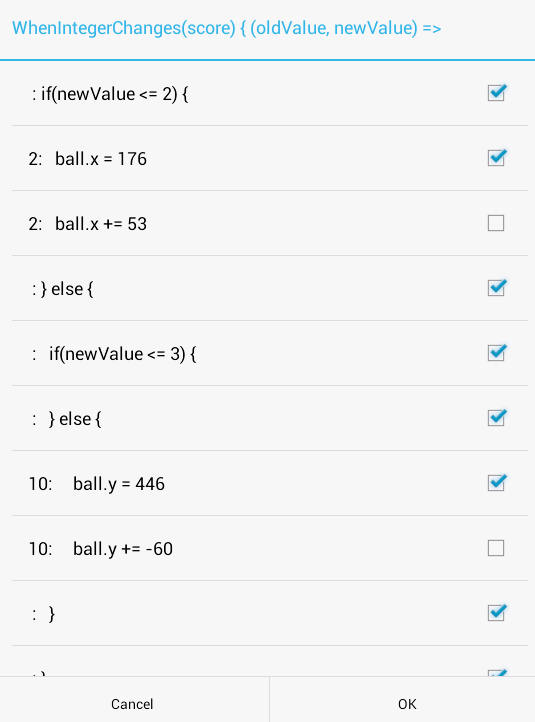
\includegraphics[height=5in]{captures/ifthenelse}}
\caption{Expanding the code to let the user choose its
specification\label{ifthenelse}}
\end{figure}

\subsection{``Bootstrapping'' the code of games}

Although it is not possible to rewrite our game engine in our game
engine itself, we introduce the possibility to bootstrap the code of
created games. A game is currently saved in a valid Scala file, that uses the
game API. Once linked to the original project and recompiled, this game can be
loaded, and again modified and saved.
The trick to do bootstrapping is to add a modifiable representation of the
code such as in Figure \ref{recompiledCode}.

\begin{figure}
\begin{lstlisting}[language=scala]
WhenFingerDownOn(textBox) {
    player.angle = -90 //more: player.angle += 90
    player.velocity = 0.066f
  }.represents(List(
    ParallelExpressions(List(
      EApply(ESelect(ESelect(EIdentShape(player), "angle"),
         "$eq"),List(EConstantNumber(-90.0))),
      EApply(ESelect(ESelect(EIdentShape(player), "angle"),
         "$plus$eq"),List(EConstantNumber(90.0))))),
    ParallelExpressions(List(
      EApply(ESelect(ESelect(EIdentShape(player), "velocity"),
        "$eq"),List(EConstantNumber(0.066)))))))
\end{lstlisting}
\caption{The compiled and interpreted version of a
rule in the source code\label{recompiledCode}}
\end{figure}

\section{Game Graphical Programming Interface (GPI)}

The general way to graphically program a game is the following:

\begin{enumerate}
 \item Add shapes to the game and modify them :
 \begin{tabular}{l}
\includegraphics[scale=0.2]{captures/shapesAdd} \\
 
\includegraphics[scale=0.2]{captures/menu}\end{tabular}
 \item Launch the game \begin{tabular}{l}\label{launchGame}
 
\includegraphics[scale=0.04]{captures/timebutton2}\end{tabular}: The time elapses
  \begin{tabular}{l}
\includegraphics[scale=0.2]{captures/timebar}\end{tabular}
 \item Pause the game
 \begin{tabular}{l}
\includegraphics[scale=0.04]{captures/timebutton}\end{tabular}
 \item At any time, to make permanent changes,
 go to the beginning by pressing the back button.
 \begin{tabular}{l}
\includegraphics[scale=0.04]{captures/back}\end{tabular}
 \item Click on the ``Create Rule'' button
 \begin{tabular}{l}\includegraphics[scale=0.2]{captures/ruleEditorButton}\end{tabular}
 \item Slide the time bar to the desired moment.
 \begin{tabular}{l}
\includegraphics[scale=0.2]{captures/timebar}\end{tabular}
 \item Select the event causing the rule
 \begin{tabular}{ccc} 
\includegraphics[scale=0.8]{captures/bing} &
 
\includegraphics[scale=0.8]{captures/numbers} & 
 
\includegraphics[scale=0.8]{captures/outscreen} \\ collision &
 numbers & out of screen \\
 \multicolumn{3}{c}{ 
\includegraphics[scale=0.8]{captures/touchdownup}} \\
 touch down & move & touch up
 \end{tabular}
 \item Change the game state with the menu
 \begin{tabular}{l}
\includegraphics[scale=0.2]{captures/menu}\end{tabular}
 \item Choose the code from possibilities.
 \begin{tabular}{ccc}
 \setlength{\fboxsep}{0pt}%
 \fbox{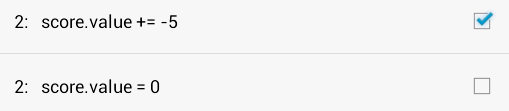
\includegraphics[scale=0.4]{captures/scoreChoose}}\end{tabular}
 \item Validate. To repeat the process, return to step \ref{launchGame} 
 \item If you want to copy a shape, just select it and create the same shape
 type.
\end{enumerate}


\section{Graphically programmed Examples}

\subsection{Fibonacci sequence}

It is simple to implement a simple interactive Fibonacci sequence. The way it
works is the following: when we press on the first score, it goes
through the sequence. When we press on the last score, it goes through the
sequence in reverse.

\begin{tabular}{l l}
\begin{minipage}{0.5\textwidth}
\begin{enumerate}
  \item Add the three scores to the game.
  \item Set their respective values to 3, 5, 8
  \item Launch the simulation
  \item Press on the 8
  \item Stop the simulation.
  \item Go back in time, select the touchdown event on 8
  \item Modify to 5, 8, 13
  \item Select OK
  \item Relaunch the simulation
  \item Press on the 5
  \item Stop the simulation
  \item Go back in time, select the touchdown event on 5
  \item Modify 5, 8, 13 to 3, 5, 8
  \item Select OK
\end{enumerate}
\end{minipage}
&
\begin{minipage}{0.5\textwidth}
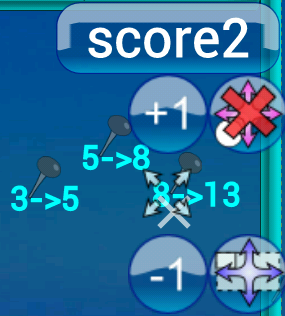
\includegraphics[width=2in]{captures/fibonacci1}
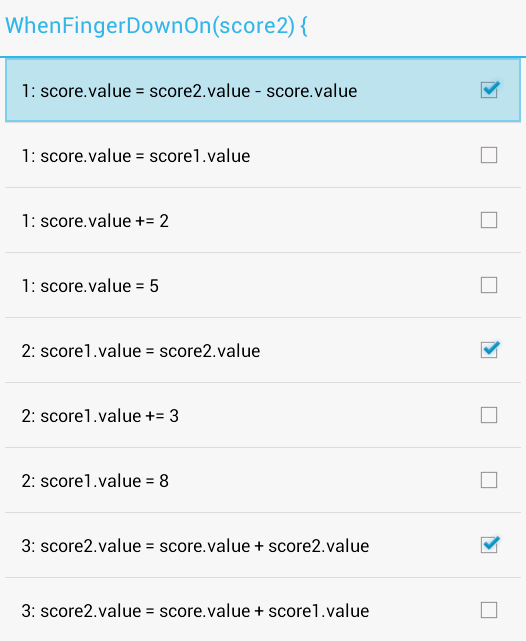
\includegraphics[width=2in]{captures/fibonacci2}
\end{minipage}
\end{tabular}

\subsection{Algorithm of Syracuse}

\begin{tabular}{l l}
\begin{minipage}{0.5\textwidth}
It is possible to graphically program a game that computes the Syracuse sequence
for any number, as well as factorial and any other functions. Here is a
screen capture of the game that computes the Syracuse sequence.

The game uses a ball to
trigger the copy of values between $3n+1$ (red) or $n/2$ (green) to top-left
orange number, depending on the parity computed in
the right-most digits. The bottom-right orange number can be customized through
up and down rectangles. To copy the value from the bottom-right orange number to
the top-left, we press the red button.
\end{minipage}
&
\begin{minipage}{0.6\textwidth}
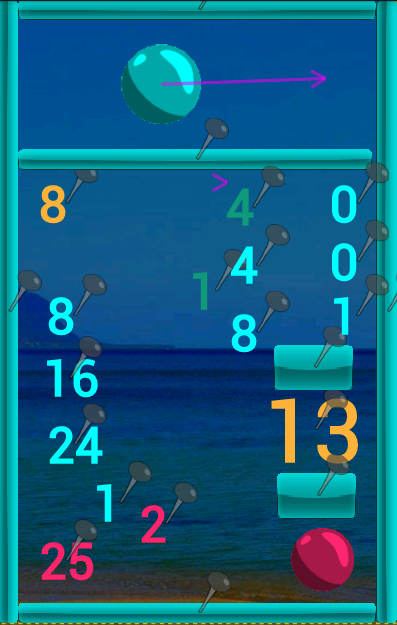
\includegraphics[width=2in]{captures/Syracuse}
\end{minipage}
\end{tabular}

\subsection{Brick-breaker}
\newcounter{tempcounter}
\hspace{-3cm}
\begin{longtable}{m{0.8\linewidth} m{2in}}
\begin{enumerate}
  \item Add a ball, a rectangle named ``block'', an integer named
``score'', an integer named ``count''
\item Change the ball's velocity towards the rectangle
\setcounter{tempcounter}{\value{enumi}}
\end{enumerate}
&   \centerline{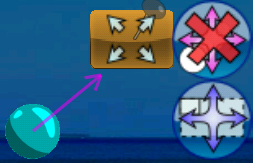
\includegraphics[width=2in]{captures/brick1}} \\
\begin{enumerate}
\setcounter{enumi}{\value{tempcounter}}
\item Launch the simulation
\item Stop after the collision
\item ``Create rule'', select the collision event, edit effects
\item Move the block apart, increment the score, increment the count, OK
\setcounter{tempcounter}{\value{enumi}}
\end{enumerate}
& \centerline{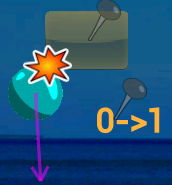
\includegraphics[width=2in]{captures/brick2}}
\\
\begin{enumerate}
\setcounter{enumi}{\value{tempcounter}}
\item Duplicate the block to make several of them
\setcounter{tempcounter}{\value{enumi}}
\end{enumerate}
& \centerline{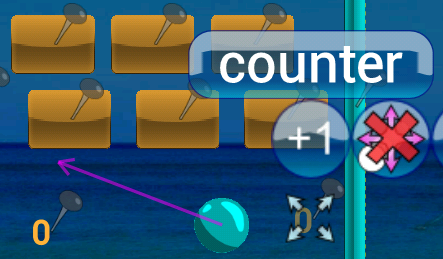
\includegraphics[width=2in]{captures/brick3}}
\\
\begin{enumerate}
\setcounter{enumi}{\value{tempcounter}}
\item Add a rectangle, rename it paddle
\item Launch the simulation from the beginning, make the gesture to move the
paddle.
\setcounter{tempcounter}{\value{enumi}}
\end{enumerate}
& \centerline{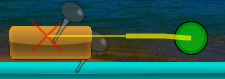
\includegraphics[width=2in]{captures/brick5}}
\\
\begin{enumerate}
\setcounter{enumi}{\value{tempcounter}}
\item Pause the simulation, select {\bf create rule}
\item Select the finger trace
\setcounter{tempcounter}{\value{enumi}}
\end{enumerate}
& \centerline{
\includegraphics[width=2in]{captures/brick6}}
\\
\begin{enumerate}
\setcounter{enumi}{\value{tempcounter}}
\item Move the paddle about approximately the same amount.
\setcounter{tempcounter}{\value{enumi}}
\end{enumerate}
&
\centerline{
\includegraphics[width=2in]{captures/brick7}}
\\
\begin{enumerate}
\setcounter{enumi}{\value{tempcounter}}
\item Confirm the rule.
\setcounter{tempcounter}{\value{enumi}}
\end{enumerate}
&
\centerline{
\includegraphics[width=2in]{captures/brick8}}
\\
\begin{enumerate}
\setcounter{enumi}{\value{tempcounter}}
\item Add a text displaying ``Game over'' in the middle, make it invisible
\item Make the ball go down and set up the velocity towards the wall below the
paddle.
\item Launch the simulation. After the collision, stop
\item Create rule, select the collision event
\item Make the ``Game over'' textbox visible
\item Make the ball to stop moving. Confirm the rule
\setcounter{tempcounter}{\value{enumi}}
\end{enumerate}
&
\centerline{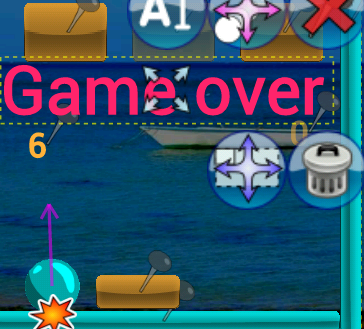
\includegraphics[width=2in]{captures/brick9}}
\\
\begin{enumerate}
\setcounter{enumi}{\value{tempcounter}}
\item Go back to the beginning
\item Make a text displaying ``Victory'' in the middle, make it invisible
\item Launch the game.
\item Pause the game. Set up the count to $n-1$, where $n$ is the number of
blocks Relaunch the game.
\item After the ball hits a block, pause the game
\item Create rule, select the number change event, select condition ``When count
== $n$''
\item Make the ``Victory'' text visible. Confirm the rule.
\end{enumerate}
&

\centerline{
\includegraphics[width=2in]{captures/brick10}}
\end{longtable}

\begin{figure}
Shapes and Arenas constructors:
\begin{lstlisting}[language=scala]
Shape
- Rectangular
  - Rectangle(x, y, width, height)
  - IntegerBox(x, y, width, height, value)
  - TexBox(x, y, width, height, text)
- Circle(x, y, radius)
Arena()
\end{lstlisting}
Modifiable properties:
\begin{lstlisting}[language=scala]
shape.x : Float
shape.y : Float
shape.angle : Float
shape.velocity : Float
shape.noVelocity : Boolean // If true, the shape sticks to the game.
shape.color : Int
shape.visible : Boolean
rectangle.width : Float  // For Rectangle, IntegerBox and TexBox
rectangle.height : Float // Idem
integerbox.value : Int
textbox.text : String
\end{lstlisting}
\caption{Shape properties\label{shapeAST}}
\end{figure}

\begin{figure}
\begin{lstlisting}[language=scala]
random(number1, number2, ...) // Chooses randomly between numbers
randomInterval(number1, number2) // Chooses a number in the interval
setCurrentArena(arena) // Sets the game to display arena
//Each new frame, if the condition is met, the code is executed
WhenEver(condition) {
  codeModifyingGameState*
}
//If the finger press on the shape, the code is executed
WhenFingerDownOn(shape) { (x, y) =>
  codeModifyingGameState*
}
//If the finger is released on the shape, the code is executed
WhenFingerUpOn(shape) { (x, y) =>
  codeModifyingGameState*
}
//If the finger moves on the shape, the code is executed
WhenFingerMovesOn(shape) { (xFrom, yFrom, xTo, yTo) =>
  codeModifyingGameState*
}
//If the integer changes, the code is executed
WhenIntegerChanges(shape) { (oldValue, newValue) =>
  codeModifyingGameState*
}
//If a collision between shape1 and shape2 occurs, the code is executed
WhenCollisionBetween(shape1, shape2) {
  codeModifyingGameState*
}
//shape1 and shape2 go trough each other without testing collision
NoCollisionBetween(shape1, shape2)
//shape1 and shape2 go through each other but collision is reported 
NoCollisionEffectBetween(shape1, shape2)
\end{lstlisting}
\caption{Game API constructors and rules\label{gameAPI}}
\end{figure}

\begin{figure}
\begin{lstlisting}
class PongGame extends Game {
  /** Game static values */
  var screenWidth = 480
  var screenHeight = 750

  /** Game Layouts */
  val arena1 = Arena() named "arena1"
  val wall = Rectangle(0, 0, 25, 750) named "wall"
  wall.noVelocity = true
  wall.color = -5266352
  arena1 += wall
  val ball = Circle(125.856f, 351.699f, 35) named "ball"
  ball.velocity_x = 0.098f
  ball.velocity_y = 0.242f
  ball.color = -19655
  arena1 += ball
  ...
  val paddle = Rectangle(179.924f, 694.477f, 120, 55) named "paddle"
  paddle.noVelocity = true
  arena1 += paddle
  val score1 = IntegerBox(50, 530, 60, 60, 0) named "score1"
  score1.noVelocity = true
  arena1 += score1
  
  WhenFingerMovesOn(paddle1) { (xFrom, yFrom, xTo, yTo) =>
    paddle1.x += xTo - xFrom // 2 more
  }
  WhenFingerMovesOn(paddle) { (xFrom, yFrom, xTo, yTo) =>
    paddle.x += xTo - xFrom // 2 more
  }
  WhenEver(ball.y + ball.radius < 0) {
    ball.x = 241
    ball.y = 376
    score1.value += 1
  }
  WhenEver(ball.y - ball.radius > screenHeight) {
    ball.x = 241
    ball.y = 376
    score.value += 1
  }
}
\end{lstlisting}
\caption{Pong game API example \label{PongAPI}}
\end{figure}


%\subsection{Escape}
%\subsection{Maze}

\section{Game Application Programming Interface (API)}
The code syntax tree is Scala-like \cite{odersky_overview_2004}.
We added a few domain-specific language features to be able to efficiently
create games.

First, we have 4 available shape types and constructors, plus one constructor
for arenas, which are containers for shapes (see Figure
\ref{shapeAST}).

These constructors are called in the class constructor to create the
game. Also available are top-level functions to build rules (see figure
\ref{gameAPI}) and to modify the game state.
Figure \ref{PongAPI} shows how to use everything to create a Pong game.



\begin{figure}
\begin{lstlisting}[language=scala]
// Shape:
// The identifiers xFrom,yFrom,xTo,yTo are available only if
// the code is inside a WhenFingerMovesOn rule.
x += xTo-xFrom (*$\bigstar$*),  x += xFrom - xTo (*$\bigstar$*),
x += Constant, x = Constant,
x += yTo-yFrom (*$\bigstar$*), x += yFrom-yTo (*$\bigstar$*)
y += yTo-yFrom (*$\bigstar$*), y += yFrom - yTo (*$\bigstar$*),
y += Constant, y = Constant,
y +=  xTo-xFrom (*$\bigstar$*), y += xFrom - xTo (*$\bigstar$*)

angle = Constant, angle += Constant
velocity *= Constant, velocity = Constant

color = Integer constant
visible = Boolean constant

// Rectangular shapes
width += xTo-xFrom (*$\bigstar$*), width = Constant,
width *= Constant, width += Constant

height += yTo-yFrom (*$\bigstar$*), height = Constant,
height *= Constant, height += Constant

// Circles
radius += Constant, radius *= Constant, radius = Constant
radius += xTo-xFrom (*$\bigstar$*)

// Integer boxes
// If the code is inside a WhenIntegerChanges rule,
// then it can use the identifiers newValue, oldValue
value = newValue, value += newValue - oldValue,
value += oldValue - newValue, value = newValue / 2 if newValue % 2 == 0,
value = newValue * 2, value = newValue - oldValue,
value = oldValue - newValue, value = oldValue,
value += Constant if Constant == 1 or -1,
value = value1 + value2, value = value1 - value2,
value = value1 * value2, value = value1 / value2,
value = value1 * 2, value = value1,
value += Constant if abs(Constant) > 1, value = Constant

// Text boxes
text = text1, text = text1 + text2, text = Constant
\end{lstlisting}
\caption{The language of actions that the game engine generates
\label{actionlanguage}}
\end{figure}

\subsection{Language of actions}

When the game state is modified, the rule generator compares the modification
against the following list of possible changes (see Figure
\ref{actionlanguage}).
The expressions are sorted by decreasing priority. When there is a
star $\bigstar$, it means that the system tolerates an error margin of 40\%
between the value specified in output and the code portion.

If multiple actions are available, the code generator wrap all actions in a
parallel instruction, where only the first instance of the code is executed.
For example, if the code is to move the shape from $x = 50$ to $x = 140$, the
system will create the line $\texttt{ParallelExpressions}(x = 140, x += 90)$.


\section{Future challenges}
Such a game engine is likely to open a wide range of new concepts
related to graphical programming. We were able to identify some directions of
future research to make such products better. Here are some of them.

\subsection{Improve execution speed}
Based on the execution traces we observed, we found out where our engine speed
could be improved.
\begin{description}
\item[Faster graphics] About 10 to 30 \% of the time is spent by software
drawing.
The use of OpenGL for example would help reduce this time.
\item[Faster collision detection] About 30 to 60\% of time is currently spent
detecting collisions. Better hashmaps and a quadtree could improve the
efficiency of the current basic $O(n^2)$ algorithm.
\item[Better game storing] About 5-15 \% of time is currently spent
storing the state of the game at each time. Storing the state at longer
intervals and then recomputing physics could allow us to improve the efficiency.
\end{description}

\subsection{Improve usability}
Based on feedback, we have some ideas about how to make the game engine more user-friendly.
\begin{description}
\item[Direct rule modification] Once a rule has been written, it would be good
to be able to modify its constants by hand and to see their immediate effect in
the game. A special display of its code would make this feasible. Deleting rules
would also be a plus.
\item[Typed objects and rules] When an object is duplicated, all the rules
linked to this object are currently duplicated. Instead, we could imagine that the rules would
be based on types, not on objects. That way, we would avoid code duplication.
\item[Saving and sharing] If this game becomes popular, we should think of
saving and loading games into a specific format that is suitable to send and
share to friends.
\item[Friction, gravity and cameras] To create platform game, we would need to
add friction, gravity and cameras in the game. That would allow us to create a
broader range of games.
\item[Better color and picture management] What makes a game fun are the
pictures and animations it is displaying. To allow to use predefined pictures and animations
would make the game more interesting.
\item[Programming abstractions] To have support for arrays types and
lambda expressions would provide a step forward to make game programming more
enjoyable.
\end{description}
\section{Evaluation to come}

The evaluation of this experiment will come in a second phase. We are planning
to have students of different ages and at different instruction levels to
program or to modify an existing game. We will be able to compare several
aspects of our game engine to state-of-the-art game engines. We plan to compare
features like the speed of learning to program, the interest, the
efficiency, and the robustness of programming with our tool.

The way we are going to record the user feedback will probably be with audio
files.

\section{Conclusion}
King Pong Designer is a nice experiment that, if continued, will certainly have
long-term effects on how to teach programming.
To make everything available to the programmer allows him to faster learn
to program and to provide visual specifications. It also allows him to
obtain the result immediately, without compilation efforts.
The game engine allows the programming of a variety of 2D games, including
multi-player games. The conclusion of this graphical approach is extremely
positive.

We hope in the future to extend this game engine with other features and also
to generalize this approach to other classes of program.

\bibliography{zoterobib}

\end{document}
